\documentclass{beamer}
%pacchetti
\usepackage[T1]{fontenc}
\usepackage[utf8]{inputenc}
\usepackage{graphicx}
\usepackage[italian]{babel}
\usepackage{mathrsfs}
\usepackage{booktabs}
\usepackage{amsmath}
\usepackage{amsfonts}
\usepackage{amssymb}
\usepackage{amsbsy}
\usepackage{amsthm}
\usepackage{enumerate}
\usepackage{quoting}
\quotingsetup{font=small}
\usepackage{diagbox}
\usepackage{graphicx}
\usepackage{setspace}
\usepackage{float}
\usepackage{version}
\usepackage{multicol}
\usepackage{beamerfoils}

\usepackage[none]{hyphenat} %avoid hyphenation
\usepackage{xcolor} %to uset \textcolor
% end pacchetti

\usetheme[bgphoto]{polimi}

% Full instructions available at:
% https://github.com/elauksap/beamerthemepolimi

% Set custom font (requires to compile with XeLaTeX).
\usepackage{ifxetex}
\ifxetex
\usepackage{fontspec}
\setsansfont[Scale=0.8]{Arial}
\fi

\usepackage{lipsum}


\newcommand\mynum[1]{%
	\usebeamercolor{enumerate item}%
	\tikzset{beameritem/.style={circle,inner sep=0,minimum size=2ex,text=enumerate item.bg,fill=enumerate item.fg,font=\footnotesize}}%
	\tikz[baseline=(n.base)]\node(n)[beameritem]{#1};%
}


\title{Is Dementia predictable?}

%\subtitle{Subtitle}
\author{F. Di Filippo, E. Manfrin, E. Musiari, E. Palli}
\date{17 december 2021}



\begin{document}
	
	\begin{frame}
		\maketitle
	\end{frame}
	
	
	\begin{frame}{Dataset}
		
		Dataset Dementia and Alzheimer longitudinal
		%\vspace{0.2 cm}
		\begin{center}
			
			
			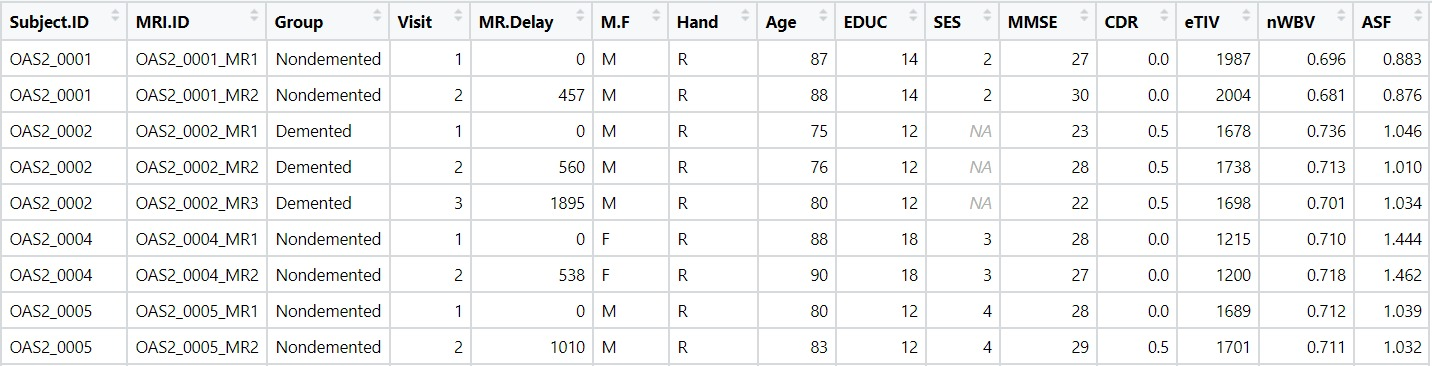
\includegraphics[width=\columnwidth]{dataset_al.jpeg}
		\end{center}
		
		
		where SES is Socioeconomic Status, MMSE is Mini Mental State Examination, CDR is Clinical Dementia Rating, eTIV is Estimated Total Intracranial Volume, nWBV is Normalize Whole Brain Volume and ASF is Atlas Scaling Factor.
		
		\vspace{0.1 cm}
		Source: Kaggle
		
		
	\end{frame}
	
	\begin{frame}{Problem of Correlation}
		We tried to solve the problem of correlation using the PCA method.
		
	\end{frame}
	
	\begin{frame}{Analysis Male VS Female}
		VARIABLE TAKEN INTO CONSIDERATION	$[Age,EDUC,MMSE,eTIV,nWBV,ASF]$ 
	$$
	H_0: \mathbf{Y}_{female} \overset{d}{=} \mathbf{Y}_{male}\;vs\;H_1:\mathbf{Y}_{female} \overset{d}{\neq} \mathbf{Y}_{male}
	$$
	 
	% hist: histmvsf
	% pvalue: non mi viene la linea verde
	$pvalue= 0 $
	\end{frame}
		\begin{frame}{Demented VS Nondemented (1) }
		$$
	H_0: \mathbf{Y}_{Demented} \overset{d}{=} \mathbf{Y}_{Non Demented}\;vs\;H_1:\mathbf{Y}_{Demented} \overset{d}{\neq} \mathbf{Y}_{Non Demented}
	$$
	
 	% hist: histdemvsnondem
 	% pvalue:  histdemvsnondem
 	$pvalue= 0.9 $
	\end{frame}
	
	\begin{frame}{Demented VS Nondemented only Male(2)}
	$$
	H_0: \mathbf{M}_{Demented} \overset{d}{=} \mathbf{M}_{Non Demented}\;vs\;H_1:\mathbf{M}_{Demented} \overset{d}{\neq} \mathbf{M}_{Non Demented}
	$$
		% hist: histdvsnmale
	% pvalue: pvaluedvsnmale
	$pvalue= 0 $
	\end{frame}
	
	\begin{frame}{Demented VS Nondemented only Female (3)}
	$$
	H_0: \mathbf{F}_{Demented} \overset{d}{=} \mathbf{F}_{Non Demented}\;vs\;H_1:\mathbf{F}_{Demented} \overset{d}{\neq} \mathbf{F}_{Non Demented}
	$$
	% hist: dvsnfemale
	% pvalue: pvaluedvsnfemale
	$pvalue= 0.37 $
		
	\end{frame}
	
	
	\begin{frame}{ TWO WAYS ANOVA: EDUCATION}
 	$$ EDUC =   \mu + \alpha_i + \beta_j + \gamma_{ij} + \epsilon  $$
 	$ i ={male,female}$
 	$ j={ Demented, Non Demented }$
 	$$ \alpha= sex$$
	$$ \beta= diagnostic$$
	$$ \gamma= interaction$$
	$$
	H_0: \gamma_{ij}=0\; \;vs\;H_1:\gamma_{ij}\neq0 
	$$
	TEST STATISTIC: $ T0= F-STATISTICS $
	$p-value = 0.082 $
	at level of confidence $ 95\% $ there's no evidence to	reject $H_0$ 
	so we reduce the model
	$$ EDUC =  \mu + \alpha_i + \beta_j  + \epsilon $$
		$$
	H_0: \beta_j=0\; \;vs\;H_1:\beta_i\neq0 
	$$
	$p-value = 0.069$
	at level of confidence $ 95\% $ there's no evidence to	reject $H_0$ there's no  evidence to reject $H_0$ 
	
	$$ EDUC =  \mu + \alpha_i  $$
	
		$$
	H_0:\alpha_i=0\; \;vs\;H_1:\alpha_i\neq0
	$$
	$p-value = 0.08 $
we could say that's neither of the grouping is significant at $95\%$ 

while with parametric test at least the diagnostic division is significant
\end{frame}
	\begin{frame}{ TWO WAYS ANOVA: MMSE}
	$$ MMSE =   \mu + \alpha_i + \beta_j + \gamma_{ij} + \epsilon $$
		$ i ={male,female}$
	$ j={ Demented, Non Demented }$
	$$
	H_0: \gamma_{ij}=0\; \;vs\;H_1:\gamma_{ij}\neq0 
	$$
	TEST STATISTIC: $ T0= F-STATISTICS $
	$p-value = 0.875 $
	there's no evidence to	reject $H_0$ 
	so we reduce the model
	$$ EDUC =   \mu + \alpha_i + \beta_j  + \epsilon  $$
	$$
	H_0:\beta_j=0\; \;vs\;H_1:\beta_j\neq0 
	$$
	$p-value = 0.446$
	a there's no evidence to reject $H_0$ there's no  evidence to reject $H_0$ 
	
	$$ EDUC =  \mu + \alpha_i $$
	
	$$
	H_0: \alpha_i =0\; \;vs\;H_1:\alpha_i \neq0 
	$$
	$p-value = 0$
	there's evidence to reject $H_0 $ 
	so the most significative model is $ MMSE \sim Diagnostic$
	where Diagnostic is the division between Demented and Non Demented
	\end{frame}
	
	\begin{frame}{regression}
		
		% modello logistico e spiegare: demented and non demented e le covariate usate: ses, normal brain volume, age, mmse -> smoothing splines; cdr senza smoothing perchè pochi valori distinti
		% fittato su tutto il dataset esclusi i converted
		
		% summary, shapiro e qqplot
		
		
		
	\end{frame}
	
	\begin{frame}{regression}
		
		% prediction sui converted
		
		% prediction su alcune persone non demented (tolte dal train del modello)
		
	\end{frame}
	
	\begin{frame}{Prediction}
		
	\end{frame}
	
	\begin{frame}{Survival Analysis}
		
		\vspace{0.3 cm}
		Event: disease occurred
		
		\begin{center}
			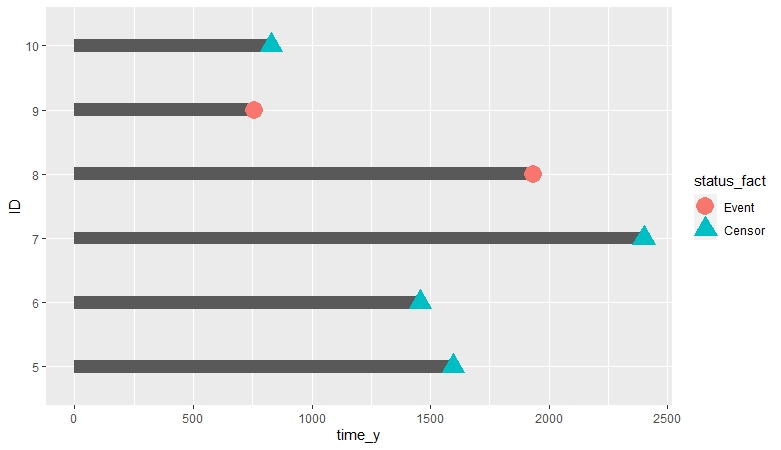
\includegraphics[width=0.9\columnwidth]{survival_plot2.jpeg}
		\end{center}
	\end{frame}
	
	\begin{frame}{Future questions}
		
	\end{frame}
	
	
\end{document}